\documentclass[10pt]{article}
\usepackage{tikz}
\usetikzlibrary{shapes.misc}
\usepackage[margin=0cm]{geometry}
\pagestyle{empty}
\tikzstyle{every node}=[cross out, draw, red]

\begin{document}

\vspace*{\fill}
\begin{center}
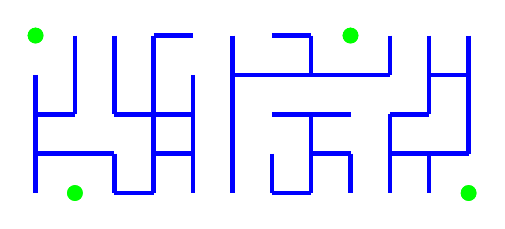
\begin{tikzpicture}[x=0.5cm, y=-0.5cm, ultra thick, blue]
% Walls
    \draw (3,0) -- (4,0);
    \draw (6,0) -- (7,0);
    \draw (5,1) -- (9,1);
    \draw (10,1) -- (11,1);
    \draw (0,2) -- (1,2);
    \draw (2,2) -- (4,2);
    \draw (6,2) -- (8,2);
    \draw (9,2) -- (10,2);
    \draw (0,3) -- (2,3);
    \draw (3,3) -- (4,3);
    \draw (7,3) -- (8,3);
    \draw (9,3) -- (11,3);
    \draw (2,4) -- (3,4);
    \draw (6,4) -- (7,4);
    \draw (0,1) -- (0,4);
    \draw (1,0) -- (1,2);
    \draw (2,0) -- (2,2);
    \draw (2,3) -- (2,4);
    \draw (3,0) -- (3,4);
    \draw (4,1) -- (4,4);
    \draw (5,0) -- (5,4);
    \draw (6,3) -- (6,4);
    \draw (7,0) -- (7,1);
    \draw (7,2) -- (7,4);
    \draw (8,3) -- (8,4);
    \draw (9,0) -- (9,1);
    \draw (9,2) -- (9,4);
    \draw (10,0) -- (10,2);
    \draw (10,3) -- (10,4);
    \draw (11,0) -- (11,3);
% Pillars
    \fill[green] (0,0) circle(0.2);
    \fill[green] (8,0) circle(0.2);
    \fill[green] (1,4) circle(0.2);
    \fill[green] (11,4) circle(0.2);
    \fill[green] (0,0) circle(0.2);
    \fill[green] (8,0) circle(0.2);
    \fill[green] (1,4) circle(0.2);
    \fill[green] (11,4) circle(0.2);
% Inner points in accessible cul-de-sacs
% Entry-exit paths without intersections
\end{tikzpicture}
\end{center}
\vspace*{\fill}
\vspace*{\fill}

\end{document}
